%\documentclass[conference]{IEEEtran}
\documentclass[10pt,conference]{IEEEtran} 
\IEEEoverridecommandlockouts
% The preceding line is only needed to identify funding in the first footnote. If that is unneeded, please comment it out.
%\usepackage{cite}
%\usepackage{amsmath,amssymb,amsfonts}
%\usepackage{algorithmic}
%\usepackage{graphicx}
%\usepackage{textcomp}
%\usepackage{xcolor}
%\def\BibTeX{{\rm B\kern-.05em{\sc i\kern-.025em b}\kern-.08em
%    T\kern-.1667em\lower.7ex\hbox{E}\kern-.125emX}}

\usepackage{epsf}
%\usepackage[bookmarks=false]{hyperref}

\usepackage{booktabs}
\usepackage{balance}
\usepackage[utf8]{inputenc}
%\usepackage{amsmath}
%\usepackage{systeme}
%\usepackage{amsfonts}
%\usepackage{amssymb}
\usepackage{graphicx}
\usepackage{listings}
\usepackage{algorithm}
\usepackage[noend]{algpseudocode}
\usepackage[utf8]{inputenc}
\usepackage[english]{babel}
\usepackage{xspace}
\usepackage{tabularx}
\usepackage{multirow}
\usepackage[table,xcdraw]{xcolor}
\usepackage{listings}
\usepackage{paralist}
\usepackage{subcaption}
%\usepackage{tikz}
\usepackage[skins]{tcolorbox}
\usepackage{enumitem,kantlipsum}
\newtcolorbox{myframe}[2][]{%
  enhanced,colback=white,colframe=black,coltitle=black,
  sharp corners,
  toprule=1.0pt,
  rightrule=0.3pt,
  leftrule=0pt,
  bottomrule=0pt,
  fonttitle=\itshape\scshape\large,
  left=0pt,right=5pt,top=5pt,bottom=3pt,
  attach boxed title to top right={yshift=-0.3\baselineskip-0.4pt,xshift=-5mm},
  boxed title style={tile,size=minimal,left=0.2mm,right=0.5mm,
    colback=white,before upper=\strut},
  title=#2,#1
}

\newcommand{\TotalPRs}{50}
\newcommand{\Responses}{42}
\newcommand{\NoAnswer}{8}

\newcommand{\Agree}{31}
\newcommand{\AgreeButNotFix}{13}

\newcommand{\Merged}{5}
\newcommand{\Approved}{13}

\newcommand{\CannotFix}{5}
\newcommand{\NotFix}{8}

\newcommand{\Disagree}{11}

\newcommand{\NoChange}{3}
\newcommand{\Override}{2}
\newcommand{\NotFixConvention}{6}

\usepackage{xspace}
\newcommand{\cf}{\hbox{\emph{cf.}}\xspace}
\newcommand{\deletia}{\ldots [deletia] \ldots}
\newcommand{\etal}{\hbox{\emph{et al.}}\xspace}
\newcommand{\eg}{\hbox{\emph{e.g.,}}\xspace}
\newcommand{\ie}{\hbox{\emph{i.e.,}}\xspace}
\newcommand{\st}{\hbox{\emph{s.t.}}\xspace}
\newcommand{\wrt}{\hbox{\emph{w.r.t.}}\xspace}
\newcommand{\viz}{\hbox{\emph{viz.}}\xspace}

\newcommand{\graphsyn}{\textsc{GraSyn}\xspace}
\newcommand{\tool}{\textsc{Phrase2Set}\xspace}
\newcolumntype{L}[1]{>{\raggedright\arraybackslash}p{#1}}
\newtheorem{observation}{Observation}
\newtheorem{property}{Property}
\newcommand{\code}[1]{{\footnotesize\textsf{#1}}}
\usepackage{amsthm}
 \definecolor{dkgreen}{rgb}{0,0.6,0}
\definecolor{gray}{rgb}{0.5,0.5,0.5}
\definecolor{mauve}{rgb}{0.58,0,0.82}

%\newcommand{\code}[1]{{\small\textsf{#1}}}
\newcommand{\algo} {Treed}
\newtheorem{Definition}{Definition}
\newtheorem{Claim}{Claim}
\newtheorem{Lemma}{Lemma}
\newtheorem{Theorem}{Theorem}
\newtheorem{Property}{Property}

\newcommand{\model} {iRTM}

\lstset{
    language={Java}, emph={},
    mathescape=false, escapeinside={/*@}{@*/},
    basicstyle=\scriptsize\sffamily,
    numberstyle=\scriptsize\sffamily,
    emphstyle=\bfseries,
    numbers=left, stepnumber=1, numbersep=-6pt,
    frame=single, xleftmargin=4pt, xrightmargin=4pt, framexleftmargin=0pt, framexrightmargin=0pt,  %xleftmargin=11pt
    columns=flexible, breaklines=true, showspaces=false, showstringspaces=true, showtabs=false, tabsize=2
}

\begin{document}

\title{Relational Topic Model for\\ Duplicate Bug Report Detection}

%\title{Incremental Relational Topic Model for\\ Duplicate Bug Report Detection}

%\author{\IEEEauthorblockN{1\textsuperscript{st} Given Name Surname}
%\IEEEauthorblockA{\textit{dept. name of organization (of Aff.)} \\
%\textit{name of organization (of Aff.)}\\
%City, Country \\
%email address or ORCID}
%\and
%\IEEEauthorblockN{2\textsuperscript{nd} Given Name Surname}
%\IEEEauthorblockA{\textit{dept. name of organization (of Aff.)} \\
%\textit{name of organization (of Aff.)}\\
%City, Country \\
%email address or ORCID}
%\and
%\IEEEauthorblockN{3\textsuperscript{rd} Given Name Surname}
%\IEEEauthorblockA{\textit{dept. name of organization (of Aff.)} \\
%\textit{name of organization (of Aff.)}\\
%City, Country \\
%email address or ORCID}
%\and
%\IEEEauthorblockN{4\textsuperscript{th} Given Name Surname}
%\IEEEauthorblockA{\textit{dept. name of organization (of Aff.)} \\
%\textit{name of organization (of Aff.)}\\
%City, Country \\
%email address or ORCID}
%\and
%\IEEEauthorblockN{5\textsuperscript{th} Given Name Surname}
%\IEEEauthorblockA{\textit{dept. name of organization (of Aff.)} \\
%\textit{name of organization (of Aff.)}\\
%City, Country \\
%email address or ORCID}
%\and
%\IEEEauthorblockN{6\textsuperscript{th} Given Name Surname}
%\IEEEauthorblockA{\textit{dept. name of organization (of Aff.)} \\
%\textit{name of organization (of Aff.)}\\
%City, Country \\
%email address or ORCID}
%}

\maketitle

\begin{abstract}
%In software development and maintenance, bug fixing is a
%time-consuming, yet unavoidable task.
A bug is occasionally reported by more than one reporters, resulting
in duplicate bug reports.  Detecting duplicate bug reports is crucial
because it helps reduce the maintenance efforts from developers as
well as provides more information in the bug fixing process. In this
paper, we propose an automatic approach to this problem. A bug report
is considered as a textual document describing one or more technical
aspects of a software system, in which some of them might be
erroneously implemented. The reports similarly describing the same
erroneous technical aspects are considered as duplicate ones. We
utilize Relational Topic Model (RTM), a probabilistic, generative
topic model, to formulate the probabilistic structures of technical
aspects in a collection of bug reports and the duplication indicators
among them. Trained with historical data including identified
duplicate reports, the model can be used to detect other
not-yet-identified duplicate ones.
%To support software evolution, we extend RTM into {\em incremental RTM
%  (iRTM)} in which the trained model can be quickly updated without
%spending a large amount of time for complete re-training when new
%reports are filed or additional duplication information is
%available.
Our empirical evaluation on several real-world systems shows that our
model outperforms the state-of-the-art approach, achieving up to 90\%
top-10 accuracy with up to x8 faster in updating its model as new
reports arrive.
\end{abstract}

%\begin{IEEEkeywords}
%component, formatting, style, styling, insert
%\end{IEEEkeywords}

\section{Introduction}
\label{intro}

%In software development and maintenance, fixing software defects
%(often called bugs) is crucial in software development to produce
%high-quality products. Bug fixing could occur during development or in
%post-release time.

Developers, testers, or users of a software system encounter the
detects and note its incorrect behaviors that do not follow the
requirements or their expectations. They could report such defects in
a bug repository that often called bug-tracking database.
%
%The process of bug fixing continues with the developers analyzing the
%phenomenon, locating the defective code, correcting them, and
%committing the fixed code to the projects' repository.
%
Users could interact with a software system in many different ways,
thus, occasionally, a bug could be filed by multiple reporters. That
leads to the {\em duplicate bug reports} for the same bugs. Because
bug reports keep being filed everyday with high pace (e.g., in
Eclipse, 3-5 new bug reports are often filed every hour), it is~vital
to detect if a new bug report is a duplicate one. This
%Detecting whether a new bug report is a duplicate one is crucial
%because it helps 
helps reduce the maintenance efforts from developers (e.g., if the bug
is already fixed) and provides additional information in the bug
fixing process (e.g., if the bug is not yet fixed).
%
However, such automated detection of duplicate bug reports is not
trivial. With different input data, usage environments or scenarios,
an erroneous behavior might expose as different phenomena (e.g.,
different outputs, traces, or screen views). Moreover, different
reporters might use different terminologies and styles, or report on
different elements to describe the same phenomena. As a result,
duplicate bug reports could be textually dissimilar.

%[Tung: we should show this in the motivating examples]

To automate the detection process of duplicate bug reports, we propose
a probabilistic approach. In our approach, each bug report is
considered as a textual document describing one or more technical
aspects/functionality of a system, in which some of them might be
erroneously implemented. The reports similarly describing the same
erroneous technical aspects are considered as duplicate
ones. Considering the technical aspects as the topics of those
text-based bug reports, we utilize Relational Topic Model
(RTM)~\cite{RTM}, a probabilistic, generative model, to formulate
their topic structures and duplication indicators. We use Gibbs
sampling~\cite{gibb} to train the model on historical data with
identified duplicate bug reports and then detect other
not-yet-identified duplicate ones.

% iRTM
%With software evolution, new reports are continually filed and new
%duplicate information could also be provided. The trained model should
%be updated with that new information. Therefore, we extend RTM into
%{\em incremental} RTM (iRTM) in which the trained model can be updated
%using a combination of a portion of existing data (historical reports
%and duplication indicators) and newly provided data (i.e., all new
%reports and additional duplication indicators). This helps save time
%on complete re-training on all old and new data, which could be very
%costly as the number of bug reports increases with a relatively high
%pace.

%
Our empirical evaluation on several large, real-world systems shows
that {\model} outperforms the state-of-the-art approach from Sun {\em
et al.}~\cite{davidlo10} in terms of both accuracy and time
efficiency. It can achieve up to 90\% top-10 accuracy, with updating
time within 0.14 seconds per new bug report on average. The updating
time for our model with new data is about 5-8 times smaller than the
re-training time of the Sun {\em et al.}'s approach
in~\cite{davidlo10}.

%
%The contributions of this paper include:

%\begin{enumerate}

%\item {\model}, an extended model from RTM to formulate the problem of
%  detecting duplicate bug reports. {\model} captures semantically the
%  technical topics in the bug reports and formulates the semantic
%  similarity measure among duplicate reports based on such topic
%  structures.

%\item Incremental algorithms for {\model} in a) training the model on
%historical bug reports and identified duplications, b) detecting
%not-yet-identified duplicate reports, and c) updating the trained
%model when new data is available. Such incremental solution supports
%well the detection of duplicate bug reports in evolving software.

%\item An empirical evaluation showing the accuracy, scalability, and
%time efficiency of {\model}.

%\end{enumerate}

%The next section presents a motivating example. Section~3 describes
%the details of our model. Section~4 presents the algorithm for
%incremental training of the model and detection of duplicate bug
%reports. Section 5 discusses our evaluation. Related work is in
%Section 6, and conclusions appear last.

\begin{figure}[t]
\sf
\scriptsize
\textbf{ID}:488105; \textbf{Reported:}:2016-02-19 08:46 EST; \\\textbf{Reporter}:Marc Dumais

\textbf{Summary}:  [memory] Traditional and Floating Point Renderings: view is initially empty

\textbf{Description}: This happens in both the Memory and Memory Browser views, for Traditional and Floating Point renderings. 

When a new Memory Browser view is created, or when a new rendering is
created in the Memory view using one of these renderings, the view is
initially not populated. It then becomes populated when a refresh
occurs, for example by re-sizing the view...
\caption{Bug report 488105~\cite{bug488105} in Eclipse project}
\label{fig:br1}
\end{figure}

%See attached screenshot for an example.

%\section{Motivating Example}
%\label{sec:example}

Let us explain an example of duplicate bug reports that motivate our
approach.
%Generally, a bug report is a record in a bug-tracking
%repository of a project, containing the descriptions on the
%bug(s).
A bug record contains the following important fields 1) a unique ID
of the report (\textbf{\sf ID}), reported date (\textbf{\sf
  ReportedDate}), the reporter (\textbf{\sf Reporter}), and a short
summary (\textbf{\sf Summary}) and a full description (\textbf{\sf
  Description}).

%\vspace{0.05in}\noindent\textbf{Observations on a bug report}
Figure~\ref{fig:br1} displays an example of an already-fixed bug
report in Eclipse project. As shown, this bug report was assigned the
ID of 488105 and reported on 02/19/2016 by Marc Dumais for a bug on
Eclipse. It described that the initial view or initial rendering for
memory browser is not populated.
%When it becomes populated when a refresh occurs.
Figure~\ref{fig:br2} presents bug report ID 493035, filed on
05/04/2016 by a different reporter, Marc-Andre Laperle. This report
was determined as reporting the same bug as in bug report 488105.

%===
%Analyzing the textual description, we have the following observations:

%\begin{enumerate}

%\item This report is about two technical functions in Eclipse:
%  \emph{memory browser} (MEM) and \emph{view management} (VM) of
%  software artifacts. In general, MEM involves the operations such as
%  \emph{create}, \emph{render}, and \emph{populate}. VM involves the
%  operations such as {\em refresh}, {\em resize}, {\em rendering},~etc.

%\item The bug occurred in the code implementing memory browsing. That
%  is, the operation {\em rendering}  on an initial view
%   was incorrectly implemented.

%\item In this bug report, the technical function MEM can be recognized
%  in its contents via the words that are relevant to memory browsing
%  such as \code{rendering}, \code{view}, \code{create}, \code{populate},
%  \code{floating}, and \code{memory}.
%  Similarly, the description also contains relevant terms to VM such
%  as \code{refresh}, \code{resize}, and \code{rendering}. Note that,
%  some words such as \code{rendering} and \code{view} are used to
%  describe both functions MEM and VM. If considering bug reports as
%  textual documents, we can view the described technical functions as
%  the \textbf{topics} of those documents.

%\end{enumerate}

\begin{figure}
\sf
\scriptsize
\textbf{ID}:Bug 493035; \textbf{Reported}: 2016-05-04 18:12 EDT; \textbf{Reporter}:Marc-Andre Laperle

\textbf{Resolution}:DUPLICATE

\textbf{Summary}: [GTK3] CDT Memory Browser initially blank

\textbf{Description}: 
Using I20160504-0035
CDT master as of today
Ubuntu 16.04 and Fedora 23 (GTK 3.18.9)
C/C++ Memory View Enhancements feature installed

1. Create a hello world C++ project
2. Start debugging
3. Open the memory browser
4. Enter main in the address field. The memory view is blank.
If the view is resized, it gets populated correctly. This works correctly in GTK2.
\caption{Bug report 493035~\cite{bug493035}, a duplication of 488105}
\label{fig:br2}
\end{figure}

%\noindent\textbf{Observations on a duplicate bug report}



%Analyzing the contents of 493035 and comparing to those of 488105, we
%can see that

%\begin{enumerate}

%\item BR 493035 also describes two aspects/functions: MEM - memory
%  browsing and VM - view management. MEM was also reported to contain
%  bug(s).

%\item The terms that are used to describe MEM are similar to those in
%  BR 488105, e.g., \code{memory}, \code{browser}, and
%  \code{initially}. The terms describing VM are somewhat similar
%  such as \code{view}, \code{resize}, and \code{populate}.

%\item BR 493035 provides additional information about the bug such as
%  the OS and the feature under which the bug occurred (Ubuntu, Fedora,
%  Memory View Enhancements, address field). It also provides the steps
%  to reproduce the bug. The text contains those additional terms. It
%  mentioned the cases that the system worked correctly such as after
%  being resized, getting populated, or in GTK2.

%\end{enumerate}

The example shows us that the detection of duplicate bug reports
could be based on their technical topics, rather than the concrete
words. Intuitively, topics are \emph{latent}, {\em
  semantic} features, while terms are \emph{visible, textual} features
of the documents. One could expect that the former would describe the
similarity of the documents more accurate than the latter. For
example, BR 488105 and BR 493035 describe the same topic, but they
might use \emph{different} terms for the same topic. In BR 493035, the
words \code{blank}, {\em debugging}, {\em view enhancements}, are used
to describe VM, while they do not appear in BR 488105.

%Thus, term-based assessment of those two documents might be less
%accurate/effective than topic-based assessment.

%Actually, using tfidf, a term-weighting scheme, we have calculate the
%cosine similarity of BR000002 and BR009779 to be 0.5???, too small to
%be considered as similar documents. In our approach, the topic-based
%probability that they are duplicated is estimated as 0.8???.
% topic EDIT in BR2 >> topic EDIT in BR1. (Buggy one!!!)

%Based on aforementioned observations, we propose to use a topic
%modeling approach for the automatic detection of duplicate bug
%reports. We utilize and adapt a probabilistic, generative topic model
%called {\em Relational Topic Model (RTM)}~\cite{RTM} for the analysis
%and inference of the hidden technical topics within bug reports and
%the relation of duplicate reports based on their topics. To support
%software evolution as new reports are constantly filed and new
%duplication information is available, we extend RTM into {\em
%incremental} RTM (iRTM) in which the trained model can be quickly
%updated without fully re-training.

%Next, let us detail our model.


\section{Modeling of Duplicate Bug Reports Detection}
%\section{Problem Formulation}
\label{formulation}

%Since the model is adapted from RTM~\cite{???}, in the text, we use
%some notations originated in~\cite{???}

We propose to use a topic modeling approach for the automatic
detection of duplicate bug reports. We utilize and adapt a
probabilistic, generative topic model called {\em Relational Topic
  Model (RTM)}~\cite{RTM} for the analysis and inference of the hidden
technical topics within bug reports and the relation of duplicate
reports based on their topics.

%\vspace{0.04in}
%\noindent\textbf{Overview.} This section describes our formulation for
%the problem of detecting duplicate bug reports. In our approach,
Each system is considered to have a number of (technical)
aspects. The bug database is considered as a collection of bug
reports. Each aspect of the system is considered as a topic of that
collection, represented via a set of certain words/terms. Each bug
report is considered as a textual document containing a number of
words/terms to report on some of those technical aspects. Among them,
some aspects might be incorrectly implemented with respect to the
system's requirements, thus, causing the bugs being reported. Two bug
reports are considered to be duplicate if they similarly describe the
same buggy topic(s). From now on, we use the terms (technical)
``aspect'' and ``topic'' interchangeably. The same treatment is for
``bug report'' and ``document'', and ``word'' and ``term''.

Since a document is a bug report, their topics with higher proportions
are more likely to be buggy or highly relevant to the buggy
topics. Other topics might have zero or very low proportion. If two
documents are duplicate, i.e. reporting the same buggy topics, their
corresponding topic proportions of those common topics would be high
in both reports. If two documents are not duplicate bug reports, the
two topic proportions might not be much similar (i.e. the distribution
values of common topics might not be high in both documents).

%
%To formulate the duplicate bug reports detection problem, we develop a
%parameterized, probabilistic, generative model. We call it
%\emph{incremental Relational Topic Model (iRTM)} because we extend the
%original RTM~\cite{RTM} for this detection problem. The key ideas of
%{\model} include:

%1) it considers bug reports as the observations which arise from a
%generative, probabilistic process with hidden variables. For this
%problem, the collection of bug reports including duplicate ones is
%modeled as to be {\em generated} by {\model} model;

%2) via training on historical data, for example the already-identified
%   as duplicate bug reports, it {\em estimates} those hidden variables
%   using posterior inference;

%3) then it situates new data into the estimated model, i.e., it will
%   predict {\em how likely a new bug report and an existing one are
%   generated by the estimated model} to determine whether they are
%   duplicate ones; and

%4) The trained model is quickly updated via our incremental algorithms
%   (Section~IV) without fully re-training as new bug reports arrive.

\begin{figure}[t]
\centering
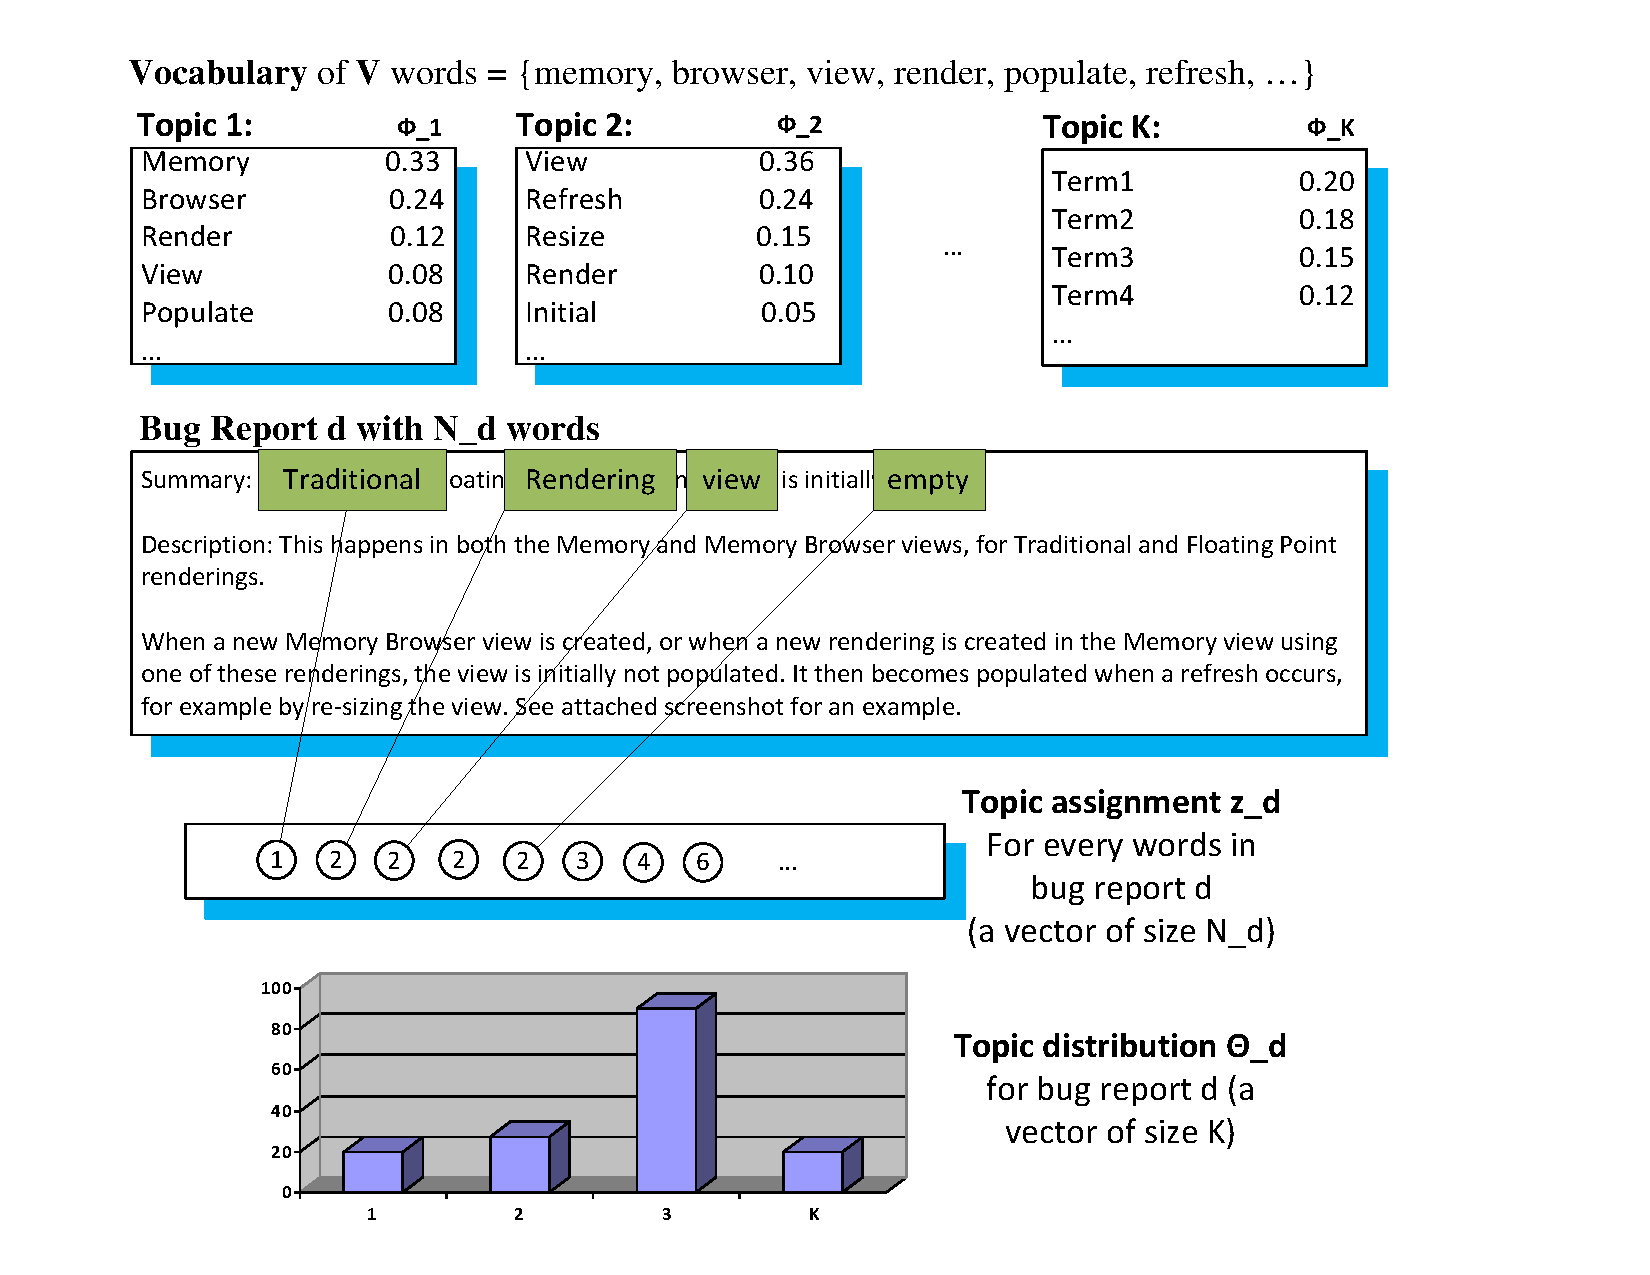
\includegraphics[width=4.2in]{irtm4}
\caption{Topic Modeling for Bug Reports~\cite{lda}}
\label{topicmodel}
\end{figure}

%\subsection{Relational Topic Modeling}


%For topic modeling in bug reports, we use LDA~\cite{lda} and adapt
%RTM~\cite{RTM}. 

%We formulate the problem of duplicate bug report detection by
%adapting RTM~\cite{RTM}.

Figure~\ref{topicmodel} shows the details.  The global
parameters include a vocabulary containing $V$ words available to be
used in the bug reports and a set of $K$ topics. The topic indexed by
$t$ ($t=1..K$) is modeled by a vector $\phi_t$ of size $V$, in which
$\phi_{t,x}$ is the probability that word $x$ in the vocabulary is
used to describe topic $t$.

A document $d$ generated by this model is considered as a sequence of
$N_d$ words, describing a mixture of such topics. The mixture, called
{\em topic distribution}, is represented by a vector $\theta_d$ of
size $K$. $\theta_{d,t}$ is the proportion of topic $t$, i.e. there
are expectedly $\theta_{d,t}*N_d$ words in document $d$ describing
topic $t$. Each position within $d$ is used to describe one topic. The
topic assignment for such positions is represented by a vector $z_d$
of size $N_d$, in which $z_{d,n}$, having value in 1..$K$, is the
index of the topic that the word $n^{th}$ in document $d$ describes.

%-------------------------------------------------------------------
\vspace{0.04in}
\noindent {\bf Duplication Indicator.} 
RTM is adapted to model the duplication relation among bug
reports. For two bug reports $d$ and $d'$, a {\em duplication
indicator} $y_{d,d'}$, will be set to 1 if they are duplicate, and 0
otherwise. Because we determine the duplication of two bug reports
based on how similarly they describe the same buggy topics, we define
a function $\psi(d,d')$ to measure the topic-based similarity of two
documents and determine the value of $y_{d,d'}$ based on
$\psi(d,d')$. That is, the higher $\psi(d,d')$ is, the higher
probability that $d$ and $d'$ are duplicate bug reports. In this
context, $\psi$ is called the {\em duplication indicating
function}. As suggested in~\cite{RTM}, we use the following function:
$$\psi(d, d') = exp({\sum\nolimits_{k=1}^K(\eta_k.\theta_{d,k}.\theta_{d',k})+
\nu})$$ in which $\eta_k$s are the weighted parameters and $\nu$ is a
smoothening parameter. As seen, this function measures the similarity of
the two documents via their topics. First, it calculates the
similarity of their topics via a weighted product of the corresponding
topic distribution vectors $\theta_d$ and $\theta_{d'}$. Then, it uses
an exponential function to amplify such similarity of those
vectors to calculate the desired topic-based similarity ($\psi(d,d')$)
between those two documents.

If two documents report the same buggy topics, their corresponding
topic distribution values of those common topics would be high in both
vectors, leading to the high weighted product and high duplication
indicating value returned in the formula via the exponential function.
If two documents are not duplicate bug reports, i.e. the distribution
values of common topics might not be high in both vectors, thus, the
weighted product and the duplication indicating value would be low.

%The correlation between this function and the duplication indicator
%could be understood intuitively as follows. Since a document is a
%bug report, their topics with higher proportions are more likely to be
%buggy or highly relevant to the buggy topics. Other topics might have
%zero or very low distribution. If two documents are duplicate,
%i.e. reporting the same buggy topics, their topic distributions might
%not be the same. However, their corresponding topic distribution
%values of those common topics would be high in both vectors, leading
%to the high weighted product and high duplication indicating value
%returned in the formula via the exponential function. Otherwise, if
%two documents are not duplicate bug reports, the two vectors might not
%be much similar (i.e. the distribution values of common topics might
%not be high in both vectors), thus, the weighted product and the
%duplication indicating value would be low.

%\vspace{0.03in}\noindent\textbf{Generation Process.}
%Formally, based on its parameters, RTM considers that the bug reports
%and their duplication indicators are generated according to the
%following probabilistic process:

%1. Choose the vocabulary of size $V$, the number of topics $K$, the
%   number of documents $M$, and the other per-collection parameters
%   $\alpha$, $\beta$, $\eta$, and $\nu$.

%2. Choose the per-topic term distributions. For each topic $t$ in
%1..$K$, draw $\phi_t$ following Dirichlet distribution
%$Dir(\beta,V)$, i.e., $\phi_t \sim Dir(\beta,V)$. Each sample of
%$Dir(\beta,V)$ is a vector of $V$ non-negative elements that are
%summed up to 1.

%3. For each document $d$ in the range of 1..$M$:

%3.1. Choose the per-document topic distribution $\theta_d$ of document
%     $d$: $\theta_d \sim Dir(\alpha, K)$. $\theta_d$ is a vector $K$
%     non-negative elements, summed up to 1, and $\theta_{d,t}$ is the
%     relative proportion of the words that are used for topic $t$ in
%     document $d$.

%3.2. Choose the size of document $N_d$ following Poisson
%     distribution as in ~\cite{RTM}.

%3.3. Choose the per-document topic assignment $z_d$ of document
%     $d$. $z_d$ is a vector of $N_d$ integer elements. The $n^{th}$
%     element is the index of the topic assigned for the $n^{th}$ word
%     in $d$. Since $d$ has topic distribution $\theta_d$,
%     $z_{d,n} \sim Multinomial(\theta_d)$.

%3.4. Generate the words $w_d$ of document $d$. $w_d$ is a vector of $N_d$
%     elements, in which $w_{d,n}$ is the index in the vocabulary of
%     the concrete word at the $n^{th}$ position of $d$. Since the
%     word at the $n^{th}$ position is assigned to topic $z_{d,n}$,
%     $w_{d,n}$ is drawn based on the per-topic term distribution
%     $\phi_{z_{d,n}}$: $w_{d,n} \sim Multinomial(\phi_{z_{d,n}})$.

%3.5. Generate the duplication indicators of document $d$ with respect
%     to other generated documents. For each generated document $d'$
%     with topic proportion $\theta_{d'}$, if $\psi(d, d')$ is sufficiently large
%     then $y_{d,d'} = 1$, otherwise $y_{d,d'} = 0$.

%Note that this is a hypothesized process from the point of view of a
%machine learning mechanism for the generation of bug reports including
%the duplicated ones. This process is used for the training and
%prediction purpose in {\model}. It does not imply a real-life process
%of bug reporting.


%\subsection{{\model} for Incremental Training and Inferring}

%Let us describe our extension to RTM for the bug report duplication
%detection. In {\model}, we use the above process to model the
%generation of the collection of bug reports including the duplicate
%ones. Therefore, we could detect duplicate bug reports by following
%step 3.5. However, we can observe only the words in bug reports,
%i.e. vector $w_d$, and some manually detected duplication indicators
%$y_{d,d'}$ for some pairs of bug reports that have been recorded in
%the history. Thus, to detect the unobserved duplication indicators of
%other pairs, we need to infer the hidden parameters of the collection
%including 1) the per-topic term distribution $\phi_t$ for the whole
%collection, 2) the per-document topic distribution $\theta_d$, and 3)
%the per-word topic assignment $z_d$ of each document. This inferring
%process must also take into account new information on reports and
%their duplications to update its inferred parameters. The reason is
%that in software evolution, new bug reports are filed continually and
%duplicate reports are also newly identified (for both old and new
%reports). Thus, there are three phases in {\model}:


%\item {\bf Initial training}.  Documents ($w_d$s) and recorded
%duplication indicators ($y_{d,d'}$s) are provided. {\model} is
%trained to get topic structures ($\phi_t$ for each $t$) of the
%collection, and that of each document ($\theta_d$ and $z_d$ for
%each~$d$).

%\vspace{0.05in}
%\item {\bf Detecting}.  In this phase, a document $d$ is provided. This
%document might be an already-filed or a newly filed bug report. We
%detect whether it is a duplicate report of another filed report. Thus,
%the model is used to infer the topic structures of the report
%($\theta_d$ and $z_d$, if needed, e.g. for a new report), and more
%importantly, its duplication indicators ($y_{d,d'}$) to all other
%documents. The inferred indicators, i.e. potential duplications, are
%reported to the users for manual verification.

%\item {\bf Updating}.  In practice, the bug reports are constantly
%  filed. New information on the duplicate reports is also provided.
%  This information includes new bug reports and duplication indicators
%  (including the indicators verified after the detecting phase, or new
%  indicators that are manually identified by users). For example, the
%  users could manually identify some new duplicate bug reports. They
% could verify some of the automatically detected duplications by our
%  tool as true duplications. The model, thus, needs to be updated with
%  newly available information. Otherwise, if the initially trained
%  model is used to process new data, that model might not fit well.

%A naive updating method is to completely re-train the model on both
%already-trained and newly available data. Since the new data is
%provided with high rate and volume, and the trained data is also of
%high volume, this naive approach would be very inefficient. On the
%other hand, if we train the model with only new data, we might miss
%the potential duplications between the new and the existing bug
%reports. Thus, our balanced approach is to select a representative
%portion of existing data to re-train with new data and use the trained
%information to update the global parameters (e.g. per-topic word
%distribution) as suggested in~\cite{canini09}. We will explain how our
%model {\model} will update its recently trained parameters such as
%$\phi_t$, $\theta_d$, $z_d$ in the next section.

%\end{enumerate}



%\section{Algorithms for initial training, detecting, and incremental updating}
\label{algorithm}

This section presents our algorithms for three aforementioned tasks:
initial training, detecting, and incremental updating. Before
presenting the algorithms (Section IV.B), let us describe a core step
in all 3 algorithms, that is, to determine the hidden (latent) topic
assignment $z_d$ of each bug report $d$ based on the provided data,
i.e. the words $w_d$ of each bug report and some recorded duplication
indicators $y_{d,d'}$s. Once the topic assignments ($z_d$s) are
inferred for all documents, we could estimate their topic proportions
($\theta_d$), the per-topic word distribution $\phi_t$ for each topic
$t$, the duplication indicating function $\psi(d,d')$, and thus, the
duplication indicators $y_{d,d'}$ of all pairs of documents.

\subsection{Sampling-based Inference of Hidden Topic Assignment}

%Direct inference of the hidden topic assignment for each document is
%intractable, thus, 

Instead of using variational inference for the hidden topic assignment
as in LDA~\cite{lda} and RTM~\cite{RTM}, we choose an approximate
approach called {\em Gibbs sampling}~\cite{gibb}. That is, the
posterior probability $P(z_d|w_d, y_{d,d'})$ is estimated by randomly
choosing the value for each element $z_{d,n}$ of $z_d$,
element-by-element, based on a distribution calculated from other
sampled values, until $P(z_d|w_d, y_{d,d'})$ is stationary. The choice
of Gibbs sampling also allows us to efficiently perform incremental
training for new data.

%A detailed description of this technique can be found in~\cite{gibb}.

%That is, we estimate the posterior probability/likelihood $P(z_d|w_d,
%y_{d,d'})$ by randomly choosing the value for each
%element $z_{d,n}$ of $z_d$, element-by-element, based on a distribution
%calculated from other sampled values, until such likelihood
%($P(z_d|w_d, y_{d,d'})$) is stationary.

%Once $z_d$ of each document is being sampled, $\theta_d$ and $\phi_t$ are also estimated based on such $z_d$s.

%In this task, the input includes: term vector $w_d$ of each bug
%report, and duplication indicators $y_{d,d'}$ of some pairs of
%manually-identified duplicate bug reports, and chosen parameters
%$\alpha, \beta, \eta$. The output includes: topic assignment vector
%$z_d$ and topic proportion $\theta_d$ of each bug report, per-topic
%term distribution $\psi_t$ of each topic, and duplication indicating
%values $\psi(\theta_d,\theta_d')$ for every pair of reports.

Specifically, the sampling-based inference of $z_d$ for each document
$d$ is as follows. The elements of $z_d$ are initially assigned with
random values. Then, each of its elements $z_{d,n}$ is sampled based
on a conditional distribution calculated from the most recent sampled
values of \emph{all other} elements, denoted by $z_{d,-n}$, and other
given information, i.e. $w_d$ and all $y_{d,d'}$s. Let us use $P(n,t)
= P(z_{d,n}=t|z_{d,-n},w_d,y_{d,d'})$ to denote the probability that
topic $t$ is assigned for the $n^{th}$ position of $d$, given
all such information. This probability depends on:

\begin{enumerate}

\item The assignments in other positions: $P(z_d[n]=t|z_d[-n])$,

\item The word $x$ chosen for position $n$: $P(w_{d,n} = x|z_{d,n} = t,z_{d,-n},w_{d,-n})$,

\item The duplication indicators of $d$ to all other documents:
   $P(z_{d,n} = t|z_{d,-n},z_{d'}, y_{d,d'})$ of all documents~$d'$.

\end{enumerate}

\vspace{0.03in}
\noindent {\bf Computation.} Those probabilities are computed as
follows:

1. $z_{d,n}$, by the generative process, is drawn based on $\theta_d$,
   while $\theta_d$ is drawn from $Dir(\alpha)$ and can be estimated
   based on $z_{d,-n}$. Let us use $\aleph(z,t)$ to denote the count
   function, i.e. the number of elements of vector $z$ having the
   value $t$. Due to the properties of Dirichlet distribution, we have
$$P_1(n,t) = P(z_{d,n} = t|z_{d,-n}) \approx \frac {\aleph(z_{d,-n},t) + \alpha} {\sum\nolimits_{k = 1}^K ({\aleph(z_{d,-n},k)} + \alpha)}$$
$$ = \frac {\aleph(z_{d,-n},t) + \alpha} {N_d - 1 + K.\alpha}$$

In other words, the topic proportion $\theta_d$ of document $d$ is
estimated by counting the assignments on $z_{d,-n}$, smoothened by
$\alpha$. Then, the probability of topic assignment $z_{d,n}$ is computed based
on such proportion.

% the ?expectation? of the distribution of $\theta_d$!!!
%(Tung: I'm not much sure about this).

2. $w_{d,n}$, by the generative process, is drawn based on $\phi_t$ if
   $z_{d,n} = t$. Let us use $w_{d,-n}(t)$ to denote the vector of words
   in $w_{d,-n}$ that are assigned to topic $t$. Due to the properties
   of Dirichlet distribution, we have
$$P_2(n,t)=P(w_{d,n}=x|z_{d,n}=t,z_{d,-n},w_{d,-n})$$ $$\approx \frac
{\aleph(w_{d,-n}(t),x) + \beta} {\sum\nolimits_{y = 1}^V
{(\aleph(w_{d,-n}(t),y) + \beta)}}= \frac {\aleph(w_{d,-n}(t),x) +
\beta} {N^{-}_{d,t} + V.\beta}$$ in which $N^{-}_{d,t}$ is the number
of words in $w_{d,-n}$ that are assigned to topic $t$.
In other words, when the position $n$ is assigned to topic $t$, we
emphasize only to the words in the document at other positions
assigned to topic $t$ (i.e. $w_{d,-n}(t)$), estimate the selection
probability of each word based on $w_{d,-n}(t)$ (smoothened by
$\beta$), and calculate the likelihood that the word $x$ has been
chosen for position $n$ (observed from data) based on that
distribution.

3. $y_{d,d'}$ is drawn based on $\psi(d, d')$ by the generative
   process. Given $z_{d,-n}$ and $z_{d'}$, we can estimate $\theta_d$
   and $\theta_d'$. Thus:
\[
\tiny
P_3(n,t,d') = P(z_{d,n} = t|z_{d,-n},z_{d'}, y_{d,d'}=1) \propto \] \[ \frac {P(y_{d,d'}=1|z_{d,n}=t, z_{d,-n},z_{d'})} {P(y_{d,d'}=1|z_{d,-n},z_d')} = \frac {\psi(d,d')} {\psi(d_{-n},d')}
\]

Since $\theta_d$ and $\theta_{d'}$ could be estimated based on $z_d$ and $z_{d'}$, by definition, $\psi(d,d') \approx exp(S)$ and $\psi(d_{-n},d') \approx exp(S')$ with

$S = {\sum_{k=1}^K(\eta_k.\frac {\aleph(z_d,k)} {N_d}. \frac {\aleph(z_{d'},k)} {N_{d'}} + \nu)}$

\noindent and

$S_{-n} = {\sum_{k=1}^K(\eta_k.\frac {\aleph(z_{d,-n},k)} {N_d}. \frac {\aleph(z_{d'},k)} {N_{d'}} + \nu}))$

\noindent Therefore, 
$$\frac {\psi(d,d')} {\psi(d_{-n},d')} = exp(S - S_{-n})
= exp({\eta_t.\frac 1 {N_d}.\frac {\aleph(z_{d'},t)} {N_{d'}}})$$

\noindent because there is only one difference between $S$ and $S_{-n}$ at position $n$ and $z_{d,n} = t$).
The formula means that, if $d$ and $d'$ are recorded as duplicate
reports, the higher proportion of topic $t$ in $d'$, the higher the
probability that a position in $d$ is assigned to topic $t$.

%[TUNG: We have the last term from reducing the formula of $\psi$.
%Note that: the topic assignments in the [tu so] and [mau so] has only a difference at for topic $t$ at location $n$].

Using all the above, we can calculate the distribution for sampling
topic assignment at each position of $d$ as:

$$P(n,t) \propto P_1(n,t).P_2(n,t). \prod_{d': y_{d,d'}=1} P_3(n,t,d')(*)$$

The last product is applied for all documents initially specified as
the duplications of $d$, i.e. all $d'$s such that $y_{d,d'} = 1$. This
is used for the pairs of reports that were recorded as duplicate
ones. For the documents having no observed duplication indicators to
$d$, we consider their indicators as un-observed, thus, ignore their
impact in topic assignment of $d$.

\subsection{Algorithms for Three Phases}

Let us describe the algorithms for three core tasks in {\model}.

%the usage of
%{\model}.

%^\vspace{0.05in}\noindent\textbf{1. Training with Initial Data}
\subsubsection{Training with Initial Data}

Using the previous core step, the initial training algorithm is as
follows:

\begin{itemize}

\item Step 1. Initialize randomly the values for all $z_d$s.

\item Step 2. For each $d$, sample $z_d$ element-by-element following
distribution (*) until it is stationary.

\item Step 3. Estimate the topic proportion of each document: $\theta_{d,t}
\approx \frac {\aleph(z_d,t)} {N_d}$.

\item Step 4. Estimate the word distribution for each topic: $\phi_{t,x}
\approx \frac {\sum_{d}{\aleph(z_d(t),x)}} {\sum_{d} {N_d(t)}}$,
i.e. count the assignments $N_d(t)$ of topic $t$ in each document $d$,
sum up for the whole collection, and estimate the proportion of
assignments using word $x$.

\end{itemize}

%\vspace{0.05in}\noindent\textbf{2. Detecting Duplicate Bug Reports}

\subsubsection{Detecting Duplicate Bug Reports}

Given a new report $d$, we need to determine if it is
duplicate of a bug report(s) in the historical data. The
detection process is as follows:

\begin{itemize}

\item Step 1. Initialize the values for $z_d$.

\item Step 2. Sample $z_d$ following the distribution (*) until it is
stationary.

\item Step 3. Estimate the topic proportion of $d$: $\theta_{d,t} \approx
\frac {\aleph(z_d,t)} {N_d}$.

\item Step 4. For any other document $d'$ in the collection, calculate the
duplication indicating function $\psi$ on the pair $(d, d')$ to infer
their duplication indicator $y_{d,d'}$.

\end{itemize}

Note that, $d$ could be a bug report in the historical data. In this
case, we could detect the not-yet-identified duplicate reports among
the filed ones, and the steps 1-3 are not needed since they were
done in the training phase.

%\vspace{0.05in}\noindent\textbf{3. Updating with Newly Available Data}

\subsubsection{Updating with Newly Available Data}

%In practice, the bug reports are constantly filed. New information on
%the duplicate reports is also provided. For example, the users could
%manually identify some new duplicate bug reports. They could verify
%some of the automatically detected duplications by our tool as true
%duplications. The model, thus, needs to be updated with this newly
%available information. Otherwise, if the initially trained model is
%used to process new data, that model might not fit well.

%because it is trained with old data, which might be totally irrelevant
%in the new data.

%A naive updating method is to completely re-train the model on both
%already-trained and newly available data. Since the new data is
%provided with high rate and volume, and the trained data is also of
%high volume, this naive approach would be very inefficient. However,
%if we train the model with only new data, we might miss the potential
%duplications between the new and the existing bug reports. Thus, our
%balanced approach is to select a representative portion of existing
%data to re-train with new data and use the trained information to
%update the global parameters (e.g. per-topic word distribution) as
%suggested in~\cite{canini09}.

Based on this strategy, our algorithm for incremental updating is as
follows. The input of our algorithm includes the input and output from
the last training step. In addition, the input also includes new data,
i.e. newly filed bug reports and newly provided duplication
indicators (could be among either recorded or new reports). The output
is similar as in the initial training phase.

\begin{itemize}

\item Step 1. Select all the existing/historical bug reports that are
indicated as duplications via the newly provided duplication indicators --
if exists.

\item Step 2. Randomly select another portion of historical bug reports
until having a total of $r\%$ of existing bug reports. When a bug report
is selected, we also select all its duplicate reports.

\item Step 3. Combine the selected bug reports and newly filed ones, and then
train the model on this data using the algorithm in Section~3.1.

\item Step 4. Re-estimate the parameters of the model.

\end{itemize}

$\theta_d$ is only re-estimated for the reports selected in
re-training. However, $\phi_t$ needs to be re-estimated for all bug
reports. This is done without re-counting the non-selected documents
by storing the counting values from the last training. For example,
let $n_0$, $n_1$, and $n_2$ are the numbers of words $x$ assigned to
topic $t$ in the last trained data, the old data selected for
retraining, and the re-trained data, respectively. The number of words
$x$ assigned to topic $t$ after retraining is $n_0 - n_1 + n_2$. Since
$n_0$ is stored, we only need to count $n_1$ and $n_2$ on the data
used for re-training, which is much smaller than the whole data.

\section{Preliminary Evaluation}
\label{eval}

%In this section, we describe our empirical evaluation on the detection
%accuracy of {\model} in comparison with the state-of-the-art,
%SVM-based approach by Sun {\em et al.}~\cite{davidlo10}. All of
%experiments were carried out on on a computer with CPU AMD Phenom II
%X4 965 3.0 GHz, 8GB RAM, and Windows~10.

%We also re-implemented the machine learning approach described in
%their paper~\cite{davidlo10} using SVM in LIBSVM tool.

%\subsection{Data Sets and Feature Extraction}

%\begin{table}[t]
%\centering
%\caption{Statistics of All Bug Report Data}
%    \begin{tabular}{lcrrr}
%    \hline
%    Project &  Time period &  Report &  Duplicate &  Term \\
%    \hline
%    Eclipse  &  06/29/2008 - 06/28/2010 & 6,100 & 981 & 22,558 \\
%    OpenOffice & 04/12/2010 - 04/10/2011 & 7,000 & 338 & 22,051 \\
%    Firefox  &  01/26/2011 - 04/11/2011 & 20,000 & 936 & 42,515 \\
%    Apache  &  11/19/2006 - 03/30/2011 & 10,000 & 494   & 34,850 \\
%    FreeDesktop &  01/25/2010 - 04/13/2011 & 10,000 & 543   & 33,068 \\
%    NetBeans    & 06/17/2010 - 04/13/2011 & 10,000 & 993 & 27,417\\
%    \hline
%    \end{tabular}%
%\label{data}
%\end{table}

%\begin{table}[t]
%\addtolength{\tabcolsep}{-3pt}
%\centering
%\small
%\caption{Statistics of All Bug Report Data}
%    \begin{tabular}{lcccccc}
%    \hline
%    Project &  Time period &  Report &  Dup  & Train & Test \\
%    \hline
%    OpenOffice & 01/01/2008 - 12/21/2010 & 31,138 & 3,371 & 200 & 3,171  \\
%    Moz. FireFox &  01/01/2010 - 12/31/2010 & 75,653 & 6,925 & 200 & 6,725 \\
%    Eclipse  &  01/01/2008 - 12/31/2008 & 45,234 & 3,080 & 200 & 2,880  \\
%    \hline
%    Apache  &  11/19/2006 - 03/30/2011 & 10,000 & 494   & 200 & 3,485 \\
%    FreeDesktop &  01/25/2010 - 04/13/2011 & 10,000 & 543   & 200 & 3,306 \\
%    NetBeans    & 06/17/2010 - 04/13/2011 & 10,000 & 993 & 200 & 2,741\\
%    \hline
%    \end{tabular}
%\label{data}
%\end{table}



%We used the same data sets of bug reports in the open-source projects
%as in REP~\cite{sun-ase11} (Table~\ref{data}). 

%Column \code{Time period} displays the time period of collected bug
%reports. Columns \code{Report} and \code{Dup} show the numbers of bug
%reports and duplicate ones, respectively. Columns \code{Train} and
%\code{Test} show the number of the duplicate bug reports used for
%training and testing, respectively. Each bug report has its unique
%ID, a summary, a description, comments, and other metadata
%(e.g., severity, priority, its reporter, creation date, etc). All
%projects are developed in a long history.  
%The information on the duplications is available in the 
%collected bug reports. 
%Each duplicate report is marked and links to its duplicate group. The
%data is used to train {\model} and ensemble weights, and then used to
%evaluate {\model}'s accuracy in detecting the duplication between a
%bug report and the duplicate bug report~groups.
%-------------------------------------------------

%We conducted an empirical evaluation of {\model} on several
%open-source systems. We collected the data from the bug repositories
%of the systems (Table~\ref{data}). Column \code{Time period} displays
%the time period of collected bug reports. Columns \code{Report} and
%\code{Duplicate} show the numbers of bug reports and duplicate ones,
%respectively.
%For Eclipse, we chose Eclipse' s platform component from October 2000
%to July 2010 with 61,110 bug reports, in which 14,020 are determined
%by Eclipse's developers as duplicate ones. For Jazz project from June
%2005 to June 2008, the total number of bug reports are 34,228, in
%which 874 of them are recorded as duplications. 
%Each bug report has its unique ID, a summary, a description, comments,
%and other metadata (e.g. severity, priority, its reporter, creation
%date, platform, etc).

%The summary and description of a bug report were merged and considered
%as a document. It then went through pre-processing such as stemming,
%and removing grammatical and stopwords, and single-occurrence words
%as in~\cite{davidlo10}.
%In our experiment, for {\model}, we extracted and merged the summary
%and description of each report, and used the merged contents as the
%document for the report. Each document was then preprocessed such as
%stemming for term normalization, and removing grammatical words
%(e.g., ``a'', ``the'', ``and'', etc.) and those terms appearing once in
%the entire corpus as in~\cite{RTM}. Tf-Idf was run to determine and
%remove the common words that appear in most of the bug reports.
%Then, all the words were collected and indexed into a vocabulary.
%After this phase, a bug report is represented as a vector of the
%indexes of its words in the vocabulary. After this phase, a bug report is
%represented as a vector of indexes of its words in the vocabulary and
%is used in the model. Duplication information among bug reports was
%also extracted from the repositories.

%In our experiment, we extracted and merged the summary and description
%of each report, and used the merged contents as the document for the
%report. Each document was then preprocessed such as stemming for term
%normalization, and removing grammatical words (e.g. ``a'', ``the'',
%``and'', etc) and those terms appearing once in the entire corpus as
%in~\cite{RTM}.
%%%This phase include stemming for term normalization, removing
%%%grammatical words (e.g. ``a'', ``the'', ``and'', etc) and those that
%%%appear once in the entire corpus or appear in almost all
%%%documents.
%Then, all the words were collected and indexed into a vocabulary.
%Column \code{Term} shows the number of extracted terms in each
%vocabulary set after pre-processing. After this phase, a bug report is
%represented as a vector of indexes of its words in the vocabulary and
%is used in the model. Duplication information among bug reports was
%also extracted from the repositories.


%%%That is, a document of bug report $d$ with $N$ words will have the
%%%form ${\bf{w}}_d=(w_{d0}, w_{d1}, ..., w_{dN})$ where $w_{dk}$ is the
%%%index of the word at position $k$ in the vocabulary.
%%%The link indicator for $d$ with another bug report $d'$ will take the
%%%value of 1 if they are duplicate, otherwise, it will take the value of
%%%0. The vectors of bug reports and the values for the link indicators
%%%were used as features in training {\model}.

%This vector and the link indicator of the duplicate reports of $d$
%with all other known bug reports $d'$, which take value of $1$ if $d$
%is a duplicate of $d'$ and $0$ otherwise, will be applied to the input
%of iRTM.

\begin{figure}[t]
\centering
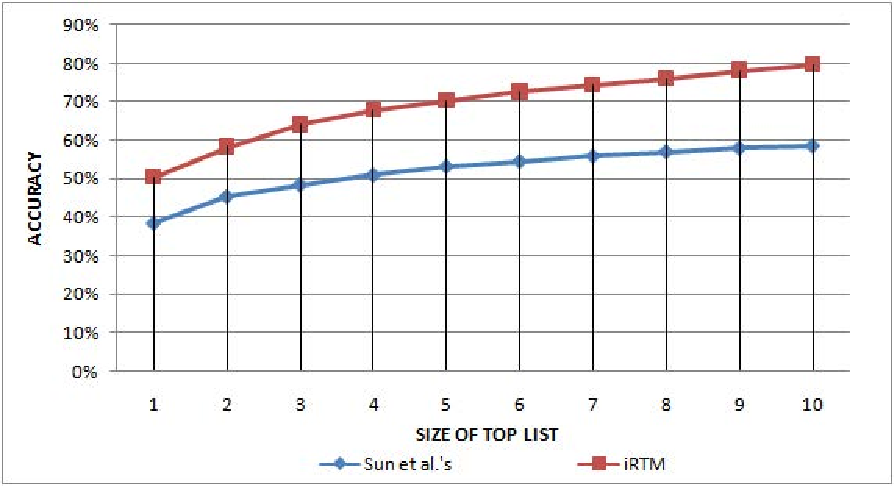
\includegraphics[width=3in]{eclipse3}
\caption{Accuracy Comparison with Different Top List Sizes}
\label{eclipse}
\end{figure}

We have conducted a preliminary evaluation on our model.
We chose the same data sets of bug reports used in
the existing work~\cite{davidlo10}. Due to the space limit, we will
not present the details of our experiment.
%In summary, our model can achieve up to 90\% top-10 accuracy, with
%updating time within 0.14 seconds per new bug report on average. The
%updating time for our model with new data is about 5-8 times smaller
%than the re-training time of the Sun {\em et al.}'s approach
%in~\cite{davidlo10}.
%Figure~\ref{eclipse} displays the accuracy result of our model in
%comparison with Sun {\em et al.}'s on Eclipse data set.
As seen in Figure~\ref{eclipse}, for a new bug report, {\bf in half of
  the detection cases, our model can correctly detect the duplication
  (if any) with just a single result}. With a list of top 5 resulting
bug reports, our model can correctly detect the duplication of a given
report in 71\% of the cases. That is, given a bug report, it can
correctly detect its duplication(s) (if any) within its top-5
recommended bug reports in almost 3 out of 4 cases. With top lists of
10 reports, it can correctly detect in 80\% of the cases. In
comparison, Sun {\em et al.}'s tool can achieve the accuracy levels at
the top lists of sizes 5 and 10 at only 53\% and 58\%,
respectively. In general, for top lists from 1-10 bug reports, {\bf
  our model achieves higher accuracy than Sun {\em et al.}'s from
  12--22\%}.




%\section{Related Work}

A related work to {\model} is the Support Vector Machine (SVM)-based
approach from Sun {\em et al.}~\cite{davidlo10}.  In the training
phase of their model, all the pairs of duplicate bug reports are
formed and considered as the positive samples. All other pairs of
non-duplicate bug reports are used as the negative samples. For each
sample (i.e. a pair of reports), a total of 54 features are
extracted. Each feature is represented by the sum of all inverse
values of the frequencies of documents containing terms or bi-grams
(i.e. two consecutive terms) that appear in the summaries and/or
descriptions of both bug reports in the sample. All positive and
negative pairs/samples are used to train and derive the parameters of
a SVM model. In the prediction phase, as a new report arrives, it
would be paired with all existing reports. Then, each pair would be
fed into the trained SVM model and be classified as positive or
negative. Positive pairs imply duplicate reports. Finally, if a new
bug report is predicted by SVM model as duplicate, it is compared
with existing bug reports to determine its master bug report.

There are key advances of {\model} over their SVM model. First, their
model is not suitable for software evolution. It cannot work in an
{\em incremental} manner. For new bug reports, their model requires
complete re-training. As the project evolves, the bug report data gets
increasingly large, the training set continually grows, and the
re-training time will keep increasing significantly. The reason is
that as more reports are added, the numbers of (negative and positive)
pairs/samples will dramatically increase due to the nature of pairing
in the SVM model. With the speed of 3-5 new bug reports per hour
(e.g. in Eclipse)~\cite{davidlo10}, their time cost of for fully
re-training is much higher than {\model}'s updating time.

%not quite practical. In contrast, {\model} can incrementally update
%its parameters in very short time as new data is available.

Another disadvantage of their approach is that, the SVM model predicts
that a new report is a duplication of multiple existing bug reports
but requires a second phase to rank which one is more likely than
others. That is, after predicting the duplication of a new bug report,
their tool performs a second phase to determine the list of potential
master reports. This adds extra computational time. In contrast,
{\model} is able to rank potential master reports based on the
probabilities of generating corresponding pairs of reports. The reason
is that {\model} treats the problem of detecting duplication reports
as a {\em ranking problem}, while their SVM-based approach considers
it as a {\em classification one}. Moreover, in contrast to our
generative model, their model is SVM, a discriminative model. The
quality of their results depends very much on the positive and
negative sets of samples. Because the percentage of duplicate bug
reports is much smaller than that of non-duplicate ones in the
project, the negative set will grow faster and their approach faces
the issue of un-balance between positive and negative samples. With
the generative approach, {\model} does not have to deal with negative
and positive sample sets. Instead, it decides the probability of
generating a pair of duplicate bug reports.

To overcome that, Sun {\em et al.}~\cite{sun-ase11} introduced REP, a
novel IR technique that extends BM25F to consider the long bug reports
and the meta-data such as the reported product, component, and
version. They showed that REP outperformed the state-of-the-art ML
approaches in both accuracy and efficiency. We did not compare with REP
because it is IR-based while we used machine learning.
%XW
%In this work, we combine BM25F with our novel topic model, T-Model, to
%address the cases where duplicate reports have different terms for the
%same technical issue. To our knowledge, DBTM is the first work in
%which topic-based features are used with IR to support the detection
%of duplicate bug reports.
%
Jalbert and Weimer~\cite{weimer08} use a binary classifier model for
predicting duplicate bug reports. They utilizes a linear regression
over {\em textual} features of bug reports computed from the
frequencies of terms in bug reports.
%%%To make a binary classifier, they specify an output value cutoff over
%%%such features that distinguishes between duplicate and non-duplicate
%%%status.
Similar to Sun {\em et al.}'s model, this model requires complete
re-training for new bug reports.
%, which is not quite efficient in practice.
Moreover, their model relies solely on {\em textual similarity}, while
{\model} focuses more on the underlying {\em technical topics} of bug
reports to determine the duplications.
%Finally, their model is discriminative, thus, facing the issue of
%unbalanced positive and negative sample sets of bug reports.

One of the first techniques to detect duplicate bug reports is Runeson
{\em et al.}'s~\cite{runeson07}. In contrast to aforementioned machine
learning (ML) approaches, Runeson {\em et al.}  utilize a natural
language processing (NLP) approach.
%The bug reports are parsed, stemmed, and the stopwords are
%removed.
Each report is modeled by a vector of textual features. The
feature of such a vector at a position corresponding to a term is
computed based on Term frequency-Inverse document
frequency~\cite{salton73}. Vector similarity is used to measure the
similarity among bug reports.
%Given a bug report under investigation, their tool returns similar bug
%reports based on the vector similarities between the new report and
%the existing ones.
Hiew~\cite{hiew06}'s approach for duplicate bug report detection is
based on information retrieval (IR) as in Runeson's. However, it uses
incremental clustering for further grouping of duplicate reports.
%is based on incremental clustering, which is quite similar to
%information retrieval. The main difference is that Hiew�s approach
%further considers the detected duplicate bug-report pairs/groups as
%clusters. Thus, when calculating similarities between a new report
%and existing bug reports, each detected cluster is considered as a
%whole rather than as several individual existing bug reports. That
%is to say, for each detected cluster, this approach will calculate one
%similarity between the new report and the detected cluster instead
%of calculating several similarities between the new report and all
%the reports in the cluster.
Comparing to those approaches, {\model} operates at a higher
abstraction level by comparing the underlying technical topics in
reports, instead of their terms. Moreover, ML approaches have been
shown to outperform NLP/IR approaches~\cite{davidlo10}. Wang {\em et
al.}~\cite{taoxie08} combine NLP with execution trace information in a
report.
%%%They utilize both Tf and Idf for textual feature extraction.
DBTM~\cite{ase12} uses a combination of IR and topic modeling.
We do not use IR in this work, therefore, we did not compare our work
with DBTM.
%Despite performance improvement, their approach is not always
%applicable in the cases where execution information considered in
%their tool is not available.
%%%and hard to collect,
%%%especially for binary programs. Sun {\em et al.}~\cite{davidlo10}
%%%reported that the percentage of reports having execution information
%%%is very low (0.83\%).

Other researchers also focus on bug reports. It is suggested that
duplicate bug reports complement to one another to help
in bug fixing~\cite{bettenburg-icsm-2008}. 
%%Bettenburg {\em et al.}~\cite{rahul08} analyzed information mismatch
%%between what developers need and what users supply to determine good
%%properties in bug reports. 
Structural information from bug reports has been shown to be
useful~\cite{bettenburg-msr08,ko06}.
%%Hooimeijer and Weimer~\cite{weimer-ase07} develop a statistic-based
%%model to automatically predict the quality of bug reports.
%Ko {\em et al.}~\cite{ko06} perform linguistic analysis on bug reports
%and suggest more structure for their contents.
Other researchers categorize bug reports based on types, quality, or
severity~\cite{rahul08,weimer-ase07,anvik06,andy-pod03,cubranic04,menzies08,bettenburg-eclipse07,weimer06,lucca02,fischer03,Sandusky04bugreport}.
%However, none of them addresses the automatic detection of duplicate
%bug reports.
From bug reports, prediction tools~\cite{weiss07,skim06} can tell
whether a bug could be resolved with certain fixing time. Approaches
for automatic assignments of bug fixers include
~\cite{anvik06,Canfora05howsoftware}.
%canfora-sac06}.
%%Other approaches aim to study the relationships among bug
%%reports~\cite{fischer03,Sandusky04bugreport}. 
Gethers and Poshyvanyk~\cite{gethers10} utilize RTM in capturing the
latent topics in classes and their relationships.





%and Whitehead claim that the time it takes to fix a
%bug is a useful software quality measure [8]. They measure
%the time taken to fix bugs in two software projects. We
%predict whether a bug will eventually be resolved as a duplicate
%and are not focused on particular resolution times or
%the total lifetime of real bugs.





%\section{Conclusions}

We propose a probabilistic model for detecting duplicate bug
reports. 
%%Each bug report is considered as a textual document about
%%technical aspects of a system. 
Duplicate bug reports are the ones similarly describing the same buggy
technical topics. We adapt RTM to formulate the probabilistic
structures of technical aspects in a collection of bug reports and the
duplication indicators among them.
%Trained with prior data on identified duplicate reports, the model is
%used to detect not-yet-identified duplicate ones. 
We also extend RTM into iRTM in which the trained model can be quickly
updated. Our evaluation on real-world systems shows that iRTM is more
accurate and time efficient than the state-of-the-art approach in Sun
{\em et al.}~\cite{davidlo10}.

%to formulate the probabilistic structures of
%technical topics in the collection of bug reports, and to find the
%indicators of the duplication among them based on those topic
%structures. 

\newpage

\balance

%\bibliographystyle{plain}
%\bibliographystyle{ACM-Reference-Format}
\bibliographystyle{IEEEtran}

\bibliography{icsme18}

%\section*{Acknowledgment}

%The preferred spelling of the word ``acknowledgment'' in America is without 
%an ``e'' after the ``g''. Avoid the stilted expression ``one of us (R. B. 
%G.) thanks $\ldots$''. Instead, try ``R. B. G. thanks$\ldots$''. Put sponsor 
%acknowledgments in the unnumbered footnote on the first page.


\end{document}
